\documentclass[english]{article}
%
\usepackage[T1]{fontenc}
\usepackage[latin9]{inputenc}
\listfiles
\usepackage[scaled]{luximono}
\usepackage{lmodern}
\usepackage{xspace,setspace}
\usepackage[bottom]{footmisc}
\usepackage{tabularx}
\usepackage{longtable}
\usepackage[NewCommands,NewParameters]{ragged2e}
\usepackage[dvipsnames]{pstricks}
\usepackage{pst-plot,pst-eps}
\usepackage{graphicx,multido}
\definecolor{hellgelb}{rgb}{1,1,0.8}
%
\def\PST{{\texttt{PSTricks}}\xspace}
\def\PDF{{\texttt{PDF}}\xspace}
\def\pst{{\texttt{pstricks}}\xspace}
\def\PS{PostScript\xspace}
\newcommand*\CMD[1]{{\UrlFont\texttt{\textbackslash #1}}}
%
\def\tIndex#1{\index{#1@{\UrlFont\texttt{#1}}}}
\def\cIndex#1{\index{#1@\CMD{#1}}}
\def\pIndex#1{\index{Parameter@\textbf{Parameter}!{\UrlFont\texttt{#1}}}}
\def\ppIndex#1{\index{Parameter@\textbf{Parameter}!{#1}}}
\def\sIndex#1{\index{Syntax@\textbf{Syntax}!\CMD{#1}}}
\def\csIndex#1{\sIndex{#1}\cIndex{#1}}
\def\PIndex#1{\index{Paket@\textbf{Paket}!\texttt{#1}}}
\def\mIndex#1{\texttt{#1}\tIndex{#1}\pIndex{#1}}
%
\pretolerance=500
\tolerance=1000 
\hbadness=3000
\vbadness=3000
\hyphenpenalty=400

\usepackage{showexpl}% not a real PSTricks package
\usepackage{babel}
\usepackage{makeidx}
\makeindex
\usepackage[dvips,colorlinks,linktocpage]{hyperref} % PDF-support
%
\renewcommand{\ttdefault}{ul9}% Luxi Mono
\lstset{keywordstyle=\small\ttfamily\bfseries} 
\lstset{language=PSTricks,moredelim=**[is][\bf\color{blue}]{�}{�}}% oder andere Begrenzer
%

\begin{document}
%
\title{\texttt{pst-eps}:\newline Export of \PST environments}
\author{Herbert Vo�%\thanks{Thanks to Lars Kotthoff and Geoff Mercer for translating this documentation!}
}
\maketitle

\begin{abstract}
It is relatively easy to save single \PST graphics as \PS files.
Important is that one
\begin{itemize}
\item puts a frame using \verb+\fbox+ around the \PST object,
\item sets the line color to \verb+white+,
\item sets \verb+\fboxsep+ to \verb+0pt+ to avoid getting any additional space,
\item chooses \verb+\pagestyle{empty}+, to suppress the page number.
\end{itemize}
\end{abstract}

\tableofcontents

\clearpage


\section{introduction}
Creating a \verb+EPS+\tIndex{EPS} file from the dvi output is possible with
%
\begin{verbatim}
dvips spirale.dvi -E -o spirale.eps
\end{verbatim}
%
which has the correct bounding box\index{bounding box} (for
figures~\ref{fig:psteps:-E} \verb+%%BoundingBox: 148 456 364 668+) on one hand
and on the other can be included as normal a graphic in the document without
problems thereafter.  Figure~\ref{fig:psteps:-E} shows a graphic created this
way and listing~\ref{lst:psteps:-E} the according source code. 

\begin{figure}[htb]
\centering
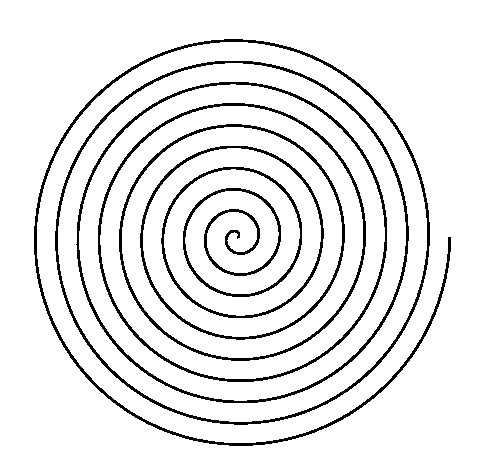
\includegraphics[scale=0.75]{spirale}
\caption{With the ``\texttt{-E}''{}- option created \texttt{EPS} file}\label{fig:psteps:-E}
\end{figure}

\begin{lstlisting}[caption={Source code for figure~\ref{fig:psteps:-E}},label={lst:psteps:-E}]
\documentclass{article}
\usepackage{pstricks}% automatically loads xcolor
\usepackage{pst-plot}
\pagestyle{empty}
\begin{document}

\color{white}% fbox invisible
\fboxsep=0pt
\fbox{%
  \begin{pspicture}(-4,-4)(4,4)
  \parametricplot[plotpoints=1000]{0}{3600}{t dup cos 1000 div mul t dup sin 1000 div mul}   
\end{pspicture}
}
\end{document}
\end{lstlisting}

With this method, one is forced to work with \verb+\fbox+, since \verb+dvips+ is
unable to determine a correct bounding box otherwise, because \verb+dvips+ does
not regard graphical elements as boundaries. As an example for this, simply
convert the above example without using \verb+\fbox+. Since \verb+\fbox+ as a
text element represents a clear boundary on text layer, \verb+dvips+ has no
problems to definitely determine the bounding box. For converting single
graphics this method is surely very efficient, but very time-consuming for a
larger number. This is where the package \verb+pst-eps+ comes in, which tries to
automate this process.

% ---------------------------------------------------------------------------------------
\section{\CMD{TeXtoEPS}}\label{sec:psteps:textoeps}
% ---------------------------------------------------------------------------------------
This macro has the task of rendering the trick with \verb+\fbox+ shown above
superfluous, and therefore give \verb+dvips+ a possiblity to correctly determine
the bounding box.

\begin{verbatim}
\TeXtoEPS%         TeX
 ... 
\endTeXtoEPS
\begin{TeXtoEPS}%  LaTeX
 ...
\end{TeXtoEPS}
\end{verbatim}
\csIndex{TeXtoEPS}
The same example as in listing~\ref{lst:psteps:-E} is picked up again, yielding
the source code in listing~\ref{lst:psteps:TeXtoEPS}.

\begin{lstlisting}[caption={Alternative source code to figure~\ref{fig:psteps:-E}},label={lst:psteps:TeXtoEPS}]
\documentclass{article}
\usepackage{pst-eps}
\usepackage{pst-plot}
\pagestyle{empty}
\begin{document}

\begin{TeXtoEPS}
  \begin{pspicture}(-3.7,-3.7)(3.7,3.7)
    \parametricplot[plotpoints=1000]{0}{3600}{t dup cos 1000 div mul t dup sin 1000 div mul}   
  \end{pspicture}
\end{TeXtoEPS}

\end{document}
\end{lstlisting}

Again the \verb+DVI+ file is converted with \verb+dvips+ as described above,
whereas this time a correct bounding box is yielded: \verb+%%BoundingBox: 71 509 286 721+,
which differs only in absolute, but not in relative values from the values given
above.



% ---------------------------------------------------------------------------------------
\section{\CMD{PSTtoEPS}}\label{sec:psteps:pstoeps}
% ---------------------------------------------------------------------------------------
With \verb+PSTtoEPS+\csIndex{PSTtoEPS} the \PST environment can be saved in an
external file without detours.

\begin{verbatim}
\PSTtoEPS[<parameters>]{<filename>}{<graphic object>} 
\end{verbatim}

With this macro the problem of the bounding box not being determined correctly
arises again. It can be specified with according parameters (table~\ref{tab:pst-eps:parameter}) 
The file is created immediately, so that it can be read direcly afterwards as
\verb+EPS+ file, as in the following example.


\begin{center}
\PSTtoEPS[bbllx=-0.5,bblly=-0.5,bburx=5.3,bbury=3.4,
  checkfile,headers=all,makeeps=all*]{frame.eps}{%
  \psgrid[subgriddiv=0](5,3)
  \psframe[linecolor=blue,linewidth=0.1](1,1)(4,2)%
}
\includegraphics[scale=0.5]{frame}
\end{center}

\begin{lstlisting}
\psset{checkfile=true}
\PSTtoEPS[bbllx=-0.5,bblly=-0.5,bburx=5.3,bbury=3.4,
  checkfile,headers=all,makeeps=all*]{frame.eps}{%
  \psgrid[subgriddiv=0](5,3)
  \psframe[linecolor=blue,linewidth=0.1](1,1)(4,2)%
}
\includegraphics[scale=0.5]{frame}
\end{lstlisting}



% ---------------------------------------------------------------------------------------
\section{Parameters}\label{sec:psteps:parameter}
% ---------------------------------------------------------------------------------------
Table~\ref{tab:pst-eps:parameter} shows a compilation of all special parameters
valid for \verb+pst-eps+.

\begin{figure}[!t]
\caption{Summary of all parameters for \texttt{pst-eps}}\label{tab:pst-eps:parameter}
\begin{tabularx}{\linewidth}{@{}>{\ttfamily}l>{\ttfamily}l>{\ttfamily}lX@{}}
\textrm{name} & \textrm{values}  & \textrm{default} & meaning\\\hline
bbllx  &  <value[unit]> & 0pt & bounding box lower left x\\
bblly  &  <value[unit]> & 0pt & lower left y\\
bburx  &  <value[unit]> & 0pt & upper right x\\
bburx  &  <value[unit]> & 0pt & upper right y\\
makeeps & none|new|all|all* & new & none: do nothing\newline
			    	    new: create, when non exists\newline
				    all: create allways\newline
				    all*: ask before overwriting\tabularnewline
checkfile & <true|false> & false & check before overwriting\\
headerfile & <filename> & \{\}   & filename of header to include\\
headers & none|all|user & none   & none: no headers\newline
                                   all: include all PSTricks header files\newline
				   user: include only the header \texttt{headerfile}\\
GraphicsRef & <{x,y}> & \{\}     & reference point\\
Translation & <{x,y}> & \{\}     & set another origin\\
Rotation & <value> &  \{\}       & rotation angle\\
Scale & <value1 value2> &  \{\}  & scaling\\
\end{tabularx}
\end{figure}
\tIndex{bbllx}\tIndex{bblly}\tIndex{bburx}\tIndex{bbury}%
\tIndex{makeeps}\tIndex{headerfile}\tIndex{headers}\tIndex{GraphicsRef}%
\tIndex{Rotation}\tIndex{Scale}
\pIndex{bbllx}\pIndex{bblly}\pIndex{bburx}\pIndex{bbury}%
\pIndex{makeeps}\pIndex{headerfile}\pIndex{headers}\pIndex{GraphicsRef}%
\pIndex{Rotation}\pIndex{Scale}


The parameters shall not be discussed in detail here, since the package
\verb+pst-eps+ can be substituted by other possiblities meanwhile.

A practical use of \verb+pst-eps+ arises, when the calculation of single objects
requires intense processor time, for instance three dimensional objects, like
cylinders or spheres. Instead of conducting those calculation at every compile
of the document again, one could create the graphic as \verb+EPS+ file in the
first place and only read it in consequent \LaTeX{} runs.


\nocite{*}
\bgroup
\raggedright
\bibliographystyle{plain}
\bibliography{\jobname}
\egroup

\printindex


\end{document}
